\chapter{Litterature}



\section{Edge detection filters}


\begin{table}[h]
	\centering
	\caption{Laplacian filter}
	\label{tab:filter:laplacian}
	\begin{tabular}{|c|c|c|}
\hline
-1 & -1 & -1 \\ \hline
-1 & 8  & -1 \\ \hline
-1 & -1 & -1 \\ \hline
	\end{tabular}
\end{table}




\section{Noise removal filter}




\subsection{Cellular Automata algorithm}

The algorithms presented in the paper \cite{bib:filter:CA} are image noise reduction algorithms based on cellular automata. For this project, it has been decided to implement the second version of the algorithm. A cellular automaton concists of a large number of simple individuals, called cells, which have a state (e.g. "on" and "off"). During one iteration, each cell updates its state depending on its own state and on the state of the neighbor cells. Two types od neighborhooh exists : the 4-connexity (Von Neumann) and the 8-connexity (Moore) neighborhood. For this algorithm, it is the Moor neighborhood that is used. In the case of the second algorithm, each pixel will be updated by taking the average value of his 8-connexity neighborhood (him included), except the minimum and the maximum values. The \vref{fig:diagram:flowchart:CAII} explains the procedure with a flowchart.


%\begin{wrapfigure}{R}{0.4\textwidth}
\begin{figure}
	\centering
	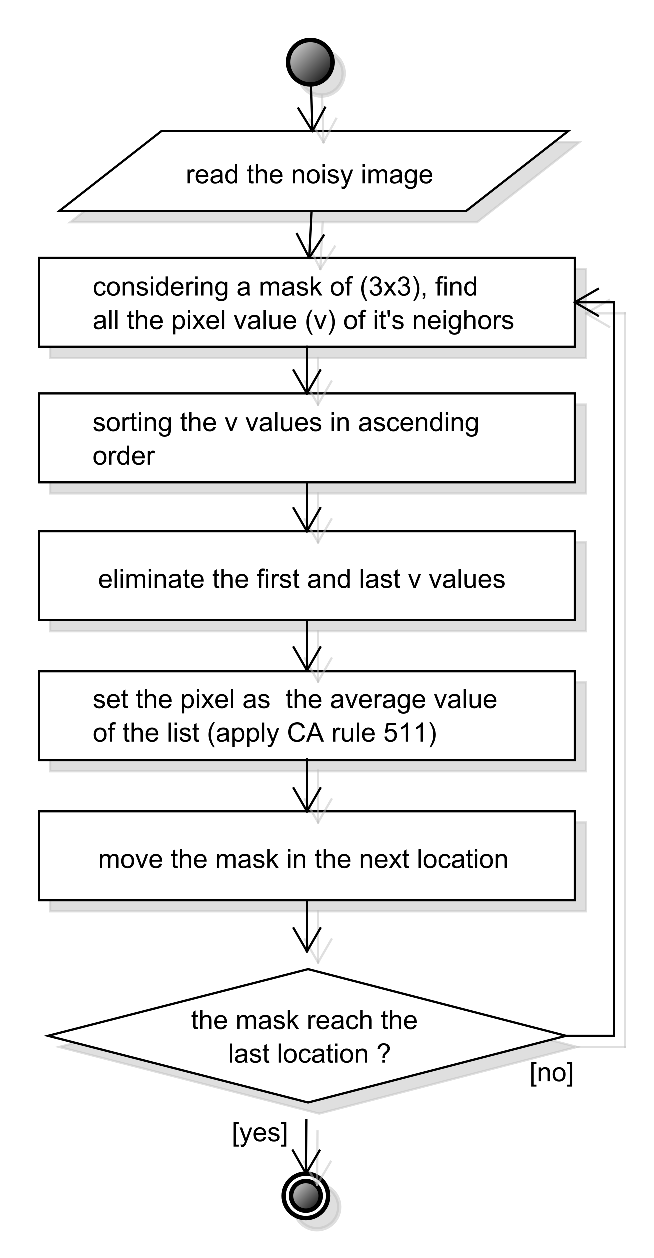
\includegraphics[width=0.4\textwidth]{images/diagrams/flowchart_CAII}
	\caption{CA II flowchart \cite{bib:filter:CA}}
	\label{fig:diagram:flowchart:CAII}
\end{figure}
%\end{wrapfigure}



\section{CLAP}

